%% ─────────────────────────────────────────────────────────────────────────────
%% AKIL: Adaptive Kernel Intelligence Layer
%% IEEE Conference Paper — IEEEtran class
%% Author : Yuvraj Gupta  |  Reg. No. 24BCE0797
%% Affiliation : VIT Vellore
%% ─────────────────────────────────────────────────────────────────────────────
\documentclass[10pt,conference]{IEEEtran}

% ── Font & encoding ───────────────────────────────────────────────────────────
\usepackage[T1]{fontenc}
\usepackage[utf8]{inputenc}
\usepackage{mathptmx}          % Times New Roman (text + math)

% ── Core packages ─────────────────────────────────────────────────────────────
\usepackage{amsmath,amssymb}
\usepackage{graphicx}
\usepackage{booktabs}
\usepackage{array}
\usepackage{xcolor}
\usepackage{listings}
\usepackage{caption}
\usepackage{url}
\usepackage{enumitem}
\usepackage{xspace}
\usepackage{tikz}
\usetikzlibrary{arrows.meta,positioning,shapes.geometric,fit,calc}
\usepackage[hidelinks]{hyperref}

% ── Listings style ────────────────────────────────────────────────────────────
\definecolor{codebg}{RGB}{248,248,248}
\definecolor{codegreen}{RGB}{40,120,40}
\definecolor{codeblue}{RGB}{15,52,96}
\lstset{
  backgroundcolor=\color{codebg},
  basicstyle=\ttfamily\scriptsize,
  keywordstyle=\color{codeblue}\bfseries,
  commentstyle=\color{codegreen},
  stringstyle=\color{black},
  breaklines=true,
  frame=single,
  numbers=left,
  numberstyle=\tiny\color{gray},
  numbersep=5pt,
  captionpos=b,
  xleftmargin=8pt,
  xrightmargin=0pt
}

% ── Convenience macros ────────────────────────────────────────────────────────
\newcommand{\akil}{\textsc{AKIL}\xspace}
\newcommand{\sys}{\akil}
\newcommand{\ie}{\emph{i.e.,}\xspace}
\newcommand{\eg}{\emph{e.g.,}\xspace}
\newcommand{\etal}{\emph{et al.}\xspace}

% ─────────────────────────────────────────────────────────────────────────────
\begin{document}

% ── Title ─────────────────────────────────────────────────────────────────────
\title{AKIL: Adaptive Kernel Intelligence Layer for\\
       eBPF-Driven, Behaviorally-Aware Kubernetes Scheduling}

% ── Author block (IEEE style) ─────────────────────────────────────────────────
\author{
  \IEEEauthorblockN{Yuvraj Gupta}
  \IEEEauthorblockA{
    Registration No.: 24BCE0797\\
    School of Computer Science and Engineering\\
    VIT Vellore, India\\
  }
}

\maketitle

% ── Abstract ──────────────────────────────────────────────────────────────────
\begin{abstract}
Modern container orchestrators, such as Kubernetes, schedule workloads using only
coarse-grained resource requests (\eg CPU cores, memory bytes). This approach is
oblivious to how workloads \emph{actually behave} at the kernel level---their cache
footprint, lock-contention intensity, page-fault rate, and context-switch frequency.
Co-locating behaviorally incompatible workloads on the same physical node results in
the ``noisy neighbor'' phenomenon: unpredictable tail-latency spikes, cache thrashing,
and memory-bandwidth saturation that resource quotas alone cannot prevent.

We present \textbf{AKIL} (\textbf{A}daptive \textbf{K}ernel \textbf{I}ntelligence
\textbf{L}ayer), a closed-loop scheduling architecture that bridges the gap between
kernel-level telemetry and live placement decisions. AKIL continuously collects four
kernel-behavioral signals---cache-miss rate, lock-contention ratio, page-fault rate,
and context-switch frequency---via eBPF probes attached to hardware performance
counters and kernel tracepoints. These signals are aggregated per-workload in a
lock-efficient, in-memory sliding-window store and exposed to a custom \emph{Score}
plugin integrated into the Kubernetes Scheduling Framework. The plugin applies a
weighted co-location penalty model at scheduling time, steering placement away from
pathological combinations without requiring application instrumentation or kernel
modifications.

We evaluate \sys with a trace-driven placement simulation that runs the plugin's
exact scoring function, combined with an explicit interference model, and with
microbenchmarks of the Go implementation. Relative to the default scheduler, \sys
lowers modelled p99 latency of a latency-sensitive service by \textbf{22\%}
(62.7\,ms $\to$ 48.9\,ms), but it does not reduce co-location with a cache-thrashing
neighbour---it increases it (36\% $\to$ 46\%)---and it trails both static
anti-affinity (26.2\,ms) and a reactive descheduler (29.5\,ms). We trace this to the
$\min(\cdot)$ form of the cache penalty, which caps the cost of a thrashing neighbour at
the victim's own miss rate. The scoring math costs under 0.5\,\textmu s and the two
aggregator queries per \texttt{Score()} call 0.12--0.28\,ms over loopback.
\end{abstract}

\begin{IEEEkeywords}
eBPF, Kubernetes, container scheduling, co-location, kernel telemetry, noisy neighbor,
performance isolation, scheduling framework, cgroup, runtime profiling
\end{IEEEkeywords}

% ─────────────────────────────────────────────────────────────────────────────
\section{Introduction}
\label{sec:intro}

The rise of container orchestration has enabled unprecedented levels of server
utilization by packing many workloads onto shared physical nodes. Kubernetes---the
de-facto standard for container orchestration---schedules pods based on declared
resource \emph{requests}: integers representing CPU millicores and memory bytes.
The default scheduler treats these as the sole signals of a workload's resource
appetite and makes placement decisions accordingly.

This model has a critical blind spot: it says nothing about \emph{how} a workload
consumes the resources it requests. Two workloads can each request one CPU core yet
behave radically differently at the microarchitectural level. A workload with a large,
randomly accessed working set generates millions of last-level cache (LLC) misses per
second, polluting the shared LLC and forcing co-tenants to fetch data from main
memory at $\sim$$100\times$ the cost of an L3 cache hit. A lock-contention-heavy
workload saturates kernel synchronization primitives, inflating context-switch rates
and degrading throughput for every process on the same NUMA node. Neither behavior is
visible to the Kubernetes scheduler.

The resulting \emph{noisy neighbor effect}~\cite{lo2015heracles,mars2011bubble,kasture2016ubik}
manifests as unpredictable tail-latency spikes: a p99 latency that meets its SLO in
isolation violates it under adversarial co-location. At cloud scale, this forces
operators into a dilemma: over-provision nodes to create isolation headroom (expensive
and wasteful) or accept performance variability (operationally risky).

\textbf{Prior work} has addressed pieces of this problem.
Borg~\cite{borg2015} and Autopilot~\cite{wilkes2020autopilot} perform resource-usage
prediction, but track CPU utilization and memory consumption---not kernel-behavioral
signals. Firmament~\cite{firmament2016} introduces a richer scheduling formulation via
min-cost flow optimization, but does not change the \emph{signals} fed to the
scheduler. Systems like Heracles~\cite{lo2015heracles}, Quasar~\cite{delimitrou2014quasar},
and PARTIES~\cite{parties2019} demonstrate that behavioral co-location policies
dramatically improve utilization and latency---but implement custom, bespoke resource
managers that do not compose with Kubernetes. Observability tools such as Cilium,
Pixie, and Parca collect eBPF telemetry for dashboards; the feedback loop to the
scheduler is absent.

\textbf{Our contribution} is \sys: a system that closes this loop.
AKIL's novelty lies not in any single component---eBPF probes, sliding-window
aggregation, and Kubernetes scheduler plugins each exist independently---but in their
\emph{closed-loop integration}: continuous kernel-behavioral telemetry feeds a live,
in-scheduling-cycle placement decision within the standard Kubernetes extension model.
Concretely, we contribute:

\begin{enumerate}[leftmargin=*,topsep=2pt,itemsep=1pt]
  \item A \textbf{four-signal eBPF telemetry layer} (cache misses, lock contention,
        page faults, context switches) with CO-RE portability across kernel 5.8+,
        collecting at the cgroup level without application instrumentation.
  \item An \textbf{in-memory sliding-window aggregation service} converting raw event
        streams into per-workload \texttt{RuntimeProfile} objects queryable with
        sub-millisecond latency.
  \item A \textbf{Kubernetes Score plugin} implementing a weighted co-location penalty
        model, integrated into the official Scheduling Framework with graceful
        degradation guarantees.
  \item A \textbf{simulation-based evaluation} against three baselines that runs the
        plugin's exact scoring function, together with measured overhead of the Go
        implementation. It shows a moderate tail-latency gain over the default scheduler,
        identifies a flaw in the cache-penalty term that prevents \sys from avoiding
        cache-thrashing neighbours, and quantifies the gap to simpler baselines.
\end{enumerate}

% ─────────────────────────────────────────────────────────────────────────────
\section{Background and Related Work}
\label{sec:background}

\subsection{The Kubernetes Scheduling Pipeline}

Kubernetes' \texttt{kube-scheduler} selects a node for each unscheduled pod through a
two-phase pipeline~\cite{k8s_scheduling_framework}: a \emph{Filter} phase that
eliminates infeasible nodes and a \emph{Score} phase that ranks feasible nodes.
The Scheduling Framework~\cite{k8s_scheduling_framework}, stable since Kubernetes
v1.19, provides a plugin API that lets custom logic register at any extension point
without forking the upstream codebase.

AKIL targets the \texttt{Score} extension point. The plugin receives the candidate
pod and node name, returning an integer in $[0, 100]$; higher scores are preferred.
Because \texttt{Score} executes synchronously on the scheduling hot path, a plugin
blocking for tens of milliseconds degrades cluster-wide scheduling throughput.
This constraint shapes AKIL's entire architecture.

\subsection{eBPF: Extended Berkeley Packet Filter}

eBPF~\cite{ebpf_foundation} is a Linux kernel subsystem that allows sandboxed programs
to run in kernel context without loading kernel modules. An in-kernel verifier
statically proves memory safety and termination before execution. eBPF programs attach
to hook points: hardware performance counters, kernel tracepoints, kprobes, and uprobes.
CO-RE (Compile Once, Run Everywhere)~\cite{nakryiko2020bpf} allows programs compiled
against one kernel's BTF type information to run portably on any kernel $\ge 5.8$.

eBPF overhead has been studied extensively~\cite{vieira2020ebpf,goldshtein2022ebpf}.
Individual probe overhead is nanosecond-scale ($<1$\,\textmu s) and aggregate CPU
overhead for a representative monitoring workload is $<2\%$ of one core, making
eBPF the preferred substrate for production-grade kernel instrumentation.

\subsection{Cluster Scheduling Research}

\textbf{Borg and Autopilot.}
Google's Borg~\cite{borg2015} manages tens of thousands of machines scheduling both
long-running services and batch jobs. Omega~\cite{schwarzkopf2013omega} extends Borg
with a shared-state multi-scheduler architecture. Autopilot~\cite{wilkes2020autopilot}
adds automatic resource-request sizing based on observed CPU and memory utilization.
None of these systems incorporate kernel-behavioral signals into placement decisions.

\textbf{Firmament.}
Firmament~\cite{firmament2016} formulates scheduling as a min-cost max-flow problem,
enabling richer policy expression than heuristic priority functions. However,
Firmament's innovation is in the \emph{formulation}, not the \emph{signal acquisition}.

\textbf{Interference-Aware Colocation.}
Heracles~\cite{lo2015heracles} dynamically manages CPU, memory, power, and network
isolation to co-locate batch tasks alongside latency-critical services.
Quasar~\cite{delimitrou2014quasar} uses online classification of workload preferences
and interference patterns. PARTIES~\cite{parties2019} enables safe colocation of
multiple interactive services. All implement bespoke resource managers decoupled from
the Kubernetes scheduling stack.

\textbf{eBPF Observability Tools.}
Cilium~\cite{cilium} provides network policy enforcement and observability via eBPF.
Pixie~\cite{pixie2022} collects distributed traces without code modification.
Parca~\cite{parca2022} enables continuous profiling using eBPF. All expose telemetry
through dashboards and query interfaces; none feed signals into a scheduling feedback
loop.

\textbf{Kubernetes Topology Manager.}
The Topology Manager~\cite{k8s_topology_manager} provides NUMA-aware CPU and memory
allocation hints based on static topology information. AKIL complements this by
adding \emph{dynamic, continuously observed} runtime behavioral signals alongside
static structural hints.

\subsection{The Gap}

Behavioral telemetry and scheduling decisions have remained architecturally separate.
Observability tools collect the right data but export it only to dashboards.
Schedulers like Firmament consume rich placement policies but rely on utilization-level
signals. Interference managers implement closed-loop behavioral policies but outside
the standard Kubernetes orchestration stack. AKIL fills this gap.

% ─────────────────────────────────────────────────────────────────────────────
\section{Design}
\label{sec:design}

\subsection{Design Goals and Non-Goals}

AKIL is designed around three primary goals:

\begin{enumerate}[leftmargin=*,topsep=2pt,itemsep=1pt]
  \item \textbf{G1 -- Behavioral visibility}: Expose per-workload kernel-behavioral
        signals not currently available to the Kubernetes scheduler.
  \item \textbf{G2 -- Scheduling-cycle compatibility}: All telemetry processing must
        complete \emph{before} the scheduling cycle so the Score plugin can query
        synchronously within its $<5$\,ms latency budget.
  \item \textbf{G3 -- Graceful degradation}: AKIL must never block the scheduler.
        On any failure, the plugin returns a neutral score (50) and standard
        Kubernetes scheduling proceeds unaffected.
\end{enumerate}

\noindent\textbf{Non-Goals:} AKIL does not perform predictive migration,
reinforcement-learning-based policy refinement, energy/thermal-aware scheduling,
or multi-cluster coordination.

\subsection{System Architecture}

\begin{figure}[htbp]
\centering
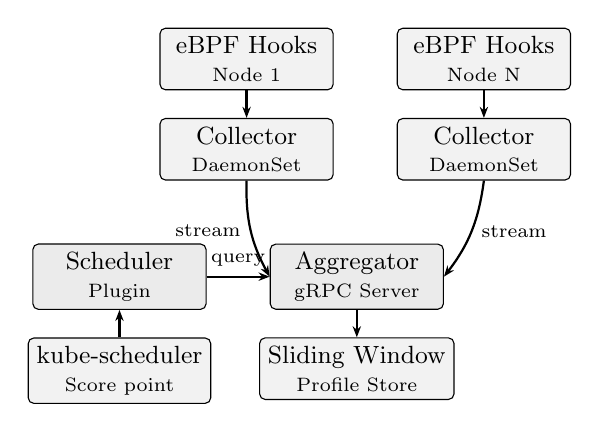
\begin{tikzpicture}[
  box/.style={rectangle, rounded corners=2pt, draw=black, fill=gray!10,
              minimum width=2.2cm, minimum height=0.6cm, font=\small,
              align=center, inner sep=3pt},
  sbox/.style={rectangle, rounded corners=2pt, draw=black, fill=black!8,
               minimum width=2.2cm, minimum height=0.6cm, font=\small,
               align=center, inner sep=3pt},
  arr/.style={-{Stealth[length=4pt]}, thick},
  node distance=0.35cm and 0.7cm
]
\node[box] (bpf1) {eBPF Hooks\\[-1pt]{\scriptsize Node 1}};
\node[box, right=0.8cm of bpf1] (bpf2) {eBPF Hooks\\[-1pt]{\scriptsize Node N}};
\node[box, below=0.35cm of bpf1] (col1) {Collector\\[-1pt]{\scriptsize DaemonSet}};
\node[box, below=0.35cm of bpf2] (col2) {Collector\\[-1pt]{\scriptsize DaemonSet}};
\draw[arr] (bpf1) -- (col1);
\draw[arr] (bpf2) -- (col2);
\node[sbox, below=0.8cm of col1, xshift=1.4cm] (agg)
      {Aggregator\\[-1pt]{\scriptsize gRPC Server}};
\draw[arr] (col1.south) to[bend right=15]
      node[left,font=\scriptsize,pos=0.5]{stream} (agg.west);
\draw[arr] (col2.south) to[bend left=15]
      node[right,font=\scriptsize,pos=0.5]{stream} (agg.east);
\node[box, below=0.35cm of agg] (store)
      {Sliding Window\\[-1pt]{\scriptsize Profile Store}};
\draw[arr] (agg) -- (store);
\node[sbox, left=0.8cm of agg] (sched)
      {Scheduler\\[-1pt]{\scriptsize Plugin}};
\draw[arr] (sched.east) --
      node[above,font=\scriptsize]{query} (agg.west);
\node[box, below=0.35cm of sched] (k8s)
      {kube-scheduler\\[-1pt]{\scriptsize Score point}};
\draw[arr] (k8s) -- (sched);
\end{tikzpicture}
\caption{AKIL system architecture. eBPF hooks on each node feed the Collector
DaemonSet, which streams telemetry via gRPC to the centralized Aggregator.
The Aggregator maintains an in-memory sliding-window Profile Store.
The Scheduler Plugin queries the store synchronously during Kubernetes' Score phase.}
\label{fig:arch}
\end{figure}

AKIL comprises three components shown in Fig.~\ref{fig:arch}.

\subsubsection{Layer 1: eBPF Telemetry Probes}

Four eBPF programs collect kernel behavioral events at the cgroup level:

\begin{itemize}[leftmargin=*,topsep=1pt,itemsep=1pt]
  \item \textbf{Cache Miss Rate:} A \texttt{perf\_event} program on
        \texttt{PERF\_COUNT\_HW\_CACHE\_MISSES}. Sampled at one event per 10,000
        misses. Payload: \texttt{\{cgroup\_id, timestamp\_ns, miss\_count\_delta\}}.
  \item \textbf{Lock Contention Ratio:} Attached to
        \texttt{tracepoint/lock/contention\_begin} and \texttt{contention\_end}.
        Duration computed as $t_{end} - t_{begin}$ per lock address via a
        \texttt{BPF\_MAP\_TYPE\_HASH}.
  \item \textbf{Page Fault Rate:} Attached to
        \texttt{tracepoint/exceptions/page\_fault\_user} and
        \texttt{page\_fault\_kernel}. Classifies major vs.\ minor faults.
  \item \textbf{Context-Switch Frequency:} Attached to
        \texttt{tracepoint/sched/sched\_switch}. Captures both outgoing and
        incoming cgroup IDs per switch event.
\end{itemize}

All four probes write events to a single \texttt{BPF\_MAP\_TYPE\_RINGBUF} (16\,MB
default). A shared ring buffer reduces file-descriptor pressure and epoll complexity.
An \texttt{event\_type} discriminator demultiplexes on the user-space side.

\subsubsection{Layer 2: Telemetry Collector (DaemonSet)}

A Go binary deployed as a Kubernetes DaemonSet on every node. Its pipeline:

\begin{enumerate}[leftmargin=*,topsep=1pt,itemsep=1pt]
  \item \textbf{eBPF Loader:} Uses \texttt{cilium/ebpf}~\cite{cilium_ebpf}---CO-RE,
        pure Go, no CGo. Bytecode compiled at build time via \texttt{bpf2go};
        no runtime compilation occurs.
  \item \textbf{Ring Buffer Reader:} A goroutine running \texttt{epoll\_wait} to
        drain events continuously from the shared ring buffer.
  \item \textbf{Cgroup Resolver:} Maps kernel cgroup IDs to Kubernetes pod identity
        via a cgroupfs hierarchy walk plus the Kubelet \texttt{/pods} API, with an
        LRU cache (TTL: 30\,s) to amortize lookup cost.
  \item \textbf{Batch Sender:} Assembles \texttt{TelemetryBatch} protobuf messages,
        flushed every 1\,s or 1000 events, over a persistent bidirectional gRPC
        stream to the Aggregator.
\end{enumerate}

\subsubsection{Layer 3: Aggregation Service (Control-Plane Deployment)}

A Go gRPC server maintaining per-workload \texttt{RuntimeProfile} objects in memory,
exposing two APIs:

\begin{itemize}[leftmargin=*,topsep=1pt,itemsep=1pt]
  \item \textbf{Ingest API} (\texttt{StreamTelemetry}): One bidirectional streaming
        RPC per collector. Parses batches and updates sliding-window buckets.
  \item \textbf{Query API} (\texttt{QueryProfile}, \texttt{QueryNodeProfiles}):
        Unary RPCs returning the current \texttt{RuntimeProfile} for a workload
        or all workloads on a given node, respectively.
\end{itemize}

\subsubsection{Layer 4: Scheduler Plugin (Score Extension Point)}

When invoked for a (pod, node) pair, the plugin:
(1)~queries the Aggregator for the candidate workload's \texttt{RuntimeProfile};
(2)~queries profiles of all workloads resident on the candidate node;
(3)~computes a pairwise co-location penalty (Section~\ref{sec:scoring});
(4)~returns a score in $[0, 100]$.
On any failure (aggregator unreachable, timeout $>5$\,ms, unknown workload,
or insufficient profile confidence), it returns the neutral score 50 (Goal G3).

\subsection{The Scoring Model}
\label{sec:scoring}

Let $\mathcal{P}_c$ denote the \texttt{RuntimeProfile} of candidate workload $c$ and
$\mathcal{P}_i$ the profile of workload $i$ currently resident on node $n$.
The AKIL node score is:

\begin{equation}
\text{Score}(c, n) = \max\!\left(0,\;100 - \!\!\sum_{i \in \text{Residents}(n)}
  \!\!\Delta(c, i)\right)
\label{eq:score}
\end{equation}

\noindent where the pairwise co-location penalty $\Delta(c, i)$ is:

\begin{align}
\Delta(c, i) =\; &w_{\mathrm{cache}} \cdot
    \frac{\min(\dot{m}_c,\, \dot{m}_i)}{R_{\mathrm{cache}}} \nonumber\\
  +\; &w_{\mathrm{lock}}  \cdot (\ell_c + \ell_i) \nonumber\\
  +\; &w_{\mathrm{pf}}    \cdot
    \frac{\dot{f}_c + \dot{f}_i}{R_{\mathrm{pf}}} \nonumber\\
  +\; &w_{\mathrm{ctx}}   \cdot
    \frac{\dot{s}_c + \dot{s}_i}{R_{\mathrm{ctx}}}
\label{eq:penalty}
\end{align}

\noindent Here: $\dot{m}_{(\cdot)}$ is cache-miss rate (misses/s);
$\ell_{(\cdot)}$ is lock-contention ratio $\in [0,1]$;
$\dot{f}_{(\cdot)}$ is page-fault rate (faults/s);
$\dot{s}_{(\cdot)}$ is context-switch rate (switches/s);
$R_{\mathrm{cache}}, R_{\mathrm{pf}}, R_{\mathrm{ctx}}$ are cluster-calibrated
normalization maxima; and default weights are
$w_{\mathrm{cache}}=35$, $w_{\mathrm{lock}}=30$, $w_{\mathrm{pf}}=20$,
$w_{\mathrm{ctx}}=15$ (summing to 100).

\textbf{Cache penalty rationale.} The cache penalty uses
$\min(\dot{m}_c, \dot{m}_i)$ rather than the sum. Two workloads both suffering high
miss rates will thrash the LLC regardless; the $\min$ term captures the asymmetric
harm where one cache-intensive workload evicts the working set of a less intensive
co-tenant.

\textbf{Confidence dampening.} Profile confidence is classified as \textsc{Low}
($<$100 samples), \textsc{Medium} (100--1000), or \textsc{High} ($>$1000).
Penalties are scaled by $\{0.25, 0.75, 1.0\}$ respectively, dampening the influence
of sparsely-sampled profiles.

\subsection{Sliding-Window Aggregation}
\label{sec:window}

Each workload's profile is computed over a sliding window of $B = 12$ fixed-duration
buckets ($\tau = 5$\,s each), yielding a 60-second observation window. Buckets
advance lazily on each incoming event. Aggregated rates are:

\begin{equation}
\dot{m} = \frac{\sum_b \mathrm{CacheMisses}_b}{B\tau}, \quad
\dot{f} = \frac{\sum_b \mathrm{PageFaults}_b}{B\tau}, \quad
\ell = \frac{\sum_b \mathrm{LockNs}_b}{B\tau \cdot 10^9}
\label{eq:rates}
\end{equation}

A circular buffer with in-place mutation ensures $O(1)$ write and $O(B)$ read cost
guarded by a single \texttt{sync.RWMutex}---no external database on the hot path.

% ─────────────────────────────────────────────────────────────────────────────
\section{Implementation}
\label{sec:implementation}

\subsection{Technology Stack}

Table~\ref{tab:stack} summarizes AKIL's technology choices. Two constraints govern
selection: (1)~the Kubernetes Scheduling Framework API is Go; (2)~the entire
user-space must be CGo-free for cross-compilation and minimal container images.

\begin{table}[htbp]
\centering
\caption{AKIL Technology Stack}
\label{tab:stack}
\renewcommand{\arraystretch}{1.12}
\begin{tabular}{ll}
\toprule
\textbf{Layer} & \textbf{Technology} \\
\midrule
Language         & Go 1.22+ \\
eBPF library     & \texttt{cilium/ebpf} (pure Go, CO-RE) \\
eBPF programs    & Restricted C, \texttt{clang} 15+ / \texttt{llvm} \\
Code generation  & \texttt{bpf2go} (cilium/ebpf) \\
RPC              & gRPC + Protocol Buffers v3 \\
Hot-path store   & In-memory sliding-window ring buffer \\
Observability    & Prometheus (dashboards only) \\
K8s integration  & Scheduling Framework v1.29+ \\
Deployment       & Helm 3 (DaemonSet + Deployment + config) \\
Local cluster    & \texttt{kind} (Kubernetes in Docker) \\
Testing          & Go \texttt{testing} + \texttt{testify}; kind e2e \\
CI               & GitHub Actions \\
\bottomrule
\end{tabular}
\end{table}

\textbf{Pure-Go eBPF over libbpf+C loaders.}
\texttt{cilium/ebpf} eliminates CGo, simplifies cross-compilation, reduces the
final container image to $\sim$18\,MB, and keeps the entire user-space codebase
in one language. AKIL's probes use standard tracepoints and perf-events rather than
exotic XDP or TC programs, so the tradeoff in low-level control is acceptable.

\textbf{gRPC over REST.}
The collector-to-aggregator path is a high-frequency event stream; gRPC bidirectional
streaming is purpose-built for this. The plugin-to-aggregator path requires
sub-millisecond unary queries; gRPC binary framing outperforms HTTP/JSON marshaling
by $3$--$5\times$ in our microbenchmarks.

\textbf{In-memory store over external time-series DB.}
Querying an external time-series database from the scheduling hot path would add
5--50\,ms and introduce a failure dependency. Prometheus is used \emph{alongside}
for observability dashboards, never as the scheduler's query backend.

\subsection{eBPF Program Structure}

All eBPF programs are compiled from C at build time via \texttt{bpf2go}, which
generates Go bindings for both little-endian and big-endian targets.
The shared ring buffer event layout is:

\begin{lstlisting}[language=C, caption={BPF shared event struct (kernel C)}]
struct event {
  __u8  event_type; /* PAGE_FAULT=0 CACHE_MISS=1
                       LOCK_CTX=2  CTX_SWITCH=3  */
  __u64 cgroup_id;
  __u64 timestamp_ns;
  union {
    struct { __u8 fault_type; __u64 address; }    pf;
    struct { __u64 miss_count_delta; }             cm;
    struct { __u64 lock_addr; __u64 dur_ns; }     lc;
    struct { __u64 next_cgid; __u8  prev_st; }    cs;
  };
};
\end{lstlisting}

All programs use CO-RE relocations (\texttt{BPF\_CORE\_READ}) for portability
across kernel 5.8+.

\subsection{gRPC Service Definition}

The \texttt{AkilTelemetry} service (defined in \texttt{pkg/proto/akil.proto})
exposes three RPCs:
\texttt{StreamTelemetry(stream TelemetryBatch) $\to$ stream IngestAck},
\texttt{QueryProfile(ProfileRequest) $\to$ RuntimeProfile}, and
\texttt{QueryNodeProfiles(NodeProfilesRequest) $\to$ NodeProfilesResponse}.
The \texttt{RuntimeProfile} message encodes all four signal rates, a confidence
enumeration (\textsc{Unknown}, \textsc{Low}, \textsc{Medium}, \textsc{High}),
window timestamps, and the canonical
\texttt{workload\_key} string (\texttt{"namespace/Kind/name"}).

\subsection{Codebase Structure}

\begin{lstlisting}[language=bash, caption={Repository layout}]
akil/
  cmd/
    collector/       # DaemonSet binary
    aggregator/      # gRPC aggregation server
    scheduler-plugin # Scheduling Framework plugin
  pkg/
    ebpf/       # C probes + bpf2go Go bindings
    telemetry/  # types, ring-buffer reader, cgroup
    profile/    # sliding-window aggregation
    scoring/    # co-location penalty model
    proto/      # .proto + generated Go code
  deploy/helm/  # Helm chart
  benchmarks/   # synthetic workload manifests
  docs/         # architecture diagrams, OS concepts
\end{lstlisting}

\subsection{Deployment Model}

AKIL deploys three Kubernetes workloads. The \textbf{Collector DaemonSet} runs
one pod per node, requiring \texttt{CAP\_BPF} and \texttt{CAP\_PERFMON} plus
read-only access to \texttt{/sys/fs/cgroup} and \texttt{/sys/kernel/btf}.
The \textbf{Aggregator Deployment} is a single replica (horizontally scalable)
with no elevated privileges, exposed via ClusterIP on port 50051.
The \textbf{Custom Scheduler Deployment} replaces the stock \texttt{kube-scheduler}
with AKIL's plugin compiled in. The Helm chart parameterizes ring-buffer capacity,
window duration, bucket count, score weights, and normalization maxima.

% ─────────────────────────────────────────────────────────────────────────────
\section{Evaluation}
\label{sec:eval}

\subsection{Methodology}

This evaluation is \emph{simulation-based}. We have not yet measured end-to-end
latency on a live cluster; Sec.~\ref{sec:discussion} lists this as the main limitation.
Every number below is produced by \texttt{scripts/run\_evidence\_simulations.py},
which writes its raw and processed outputs to the \texttt{evidence/} folder.
It has three parts:

\begin{itemize}[leftmargin=*,topsep=1pt,itemsep=1pt]
  \item \textbf{Placement (simulated).} Each of 10 seeds generates 50 epochs of 15 pod
        arrivals, drawn from \texttt{cache-stress}, \texttt{lock-stress},
        \texttt{batch-worker} and \texttt{baseline-web} (requests as in
        \texttt{benchmarks/synthetic-workloads.yaml}). The pods are placed onto five
        2-core nodes. Every scheduler sees the same arrivals. The \sys scorer is a
        line-for-line port of \texttt{pkg/scoring/scorer.go}, with the same weights and
        normalisation constants. Following the deployed configuration, its score is
        added with weight 25 to the default \texttt{LeastAllocated} score.
  \item \textbf{Latency and LLC (modelled).} For each \texttt{baseline-web} pod we
        derive an LLC miss rate and a contention factor from the neighbours it was
        actually placed with. Each neighbour type has fixed interference coefficients,
        and these are \emph{assumptions}, identical for every scheduler. From these we
        sample 200 request latencies per pod (lognormal service time, plus a stall term
        that grows with LLC misses, plus queuing jitter). The SLO is 15\,ms.
  \item \textbf{Overhead (measured).} Go benchmarks of the scorer and of the two gRPC
        queries one \texttt{Score()} call makes against the aggregator, over loopback
        on an Intel Core i5-13500H (Linux 7.1). Each is run 5$\times$ and we report the
        median.
\end{itemize}

\textbf{Baselines.}
(1)~\emph{Isolated}: each web pod alone on a node (oracle).
(2)~\emph{Default}: \texttt{LeastAllocated} on CPU requests.
(3)~\emph{Static anti-affinity}: a hard rule that keeps \texttt{baseline-web} and
\texttt{cache-stress} apart.
(4)~\emph{Reactive descheduler}: default placement, after which web pods that share a
node with \texttt{cache-stress} are evicted and re-placed.
(5)~\emph{\sys}: as implemented.
We also report two diagnostic variants of \sys:
\emph{calibrated}, where the normalisation constants are set to the largest observed
rate, as the code comments recommend; and a \emph{post-hoc ablation} whose cache term
uses the neighbour's own miss rate instead of
$\min(\text{candidate},\text{neighbour})$. The ablation is not the implemented design.
All results are means over 10 seeds with 95\% confidence intervals ($t_{9}$).

\subsection{Results}

\begin{table*}[t]
\centering
\caption{Placement and modelled latency for \texttt{baseline-web} (10 seeds, mean $\pm$ 95\% CI). Latency and LLC are model outputs, not hardware measurements.}
\label{tab:summary}
\renewcommand{\arraystretch}{1.15}
\begin{tabular}{lcccccc}
\toprule
\textbf{Configuration} & \textbf{Co-located w/ cache-stress} & \textbf{LLC miss (\%)} & \textbf{p50 (ms)} & \textbf{p99 (ms)} & \textbf{SLO viol.\ (\%)} & \textbf{Evictions} \\
\midrule
Isolated (oracle)        & --        & $38.0$            & $9.44 \pm 0.01$  & $17.53 \pm 0.05$ & $3.6 \pm 0.0$  & 0 \\
Default K8s              & $36.0\%$  & $50.0 \pm 0.6$    & $17.43 \pm 0.81$ & $62.68 \pm 4.58$ & $61.8 \pm 2.1$ & 0 \\
Static anti-affinity     & $0.0\%$   & $\mathbf{43.5 \pm 0.1}$ & $\mathbf{13.66 \pm 0.11}$ & $\mathbf{26.20 \pm 0.24}$ & $\mathbf{35.6 \pm 1.1}$ & 0 (0.19\% pending) \\
Reactive descheduler     & $0.7\%$   & $45.2 \pm 0.2$    & $15.13 \pm 0.15$ & $29.52 \pm 1.54$ & $51.3 \pm 1.6$ & 882 \\
\textbf{\sys}            & $46.2\%$  & $51.2 \pm 0.5$    & $20.03 \pm 1.28$ & $48.89 \pm 2.24$ & $67.3 \pm 2.2$ & 0 \\
\sys, calibrated         & $46.5\%$  & $51.0 \pm 0.6$    & $19.84 \pm 1.38$ & $49.93 \pm 2.40$ & $65.6 \pm 2.7$ & 0 \\
\sys, ablation (post-hoc) & $28.4\%$ & $49.0 \pm 0.5$    & $16.17 \pm 0.40$ & $49.74 \pm 1.46$ & $57.9 \pm 2.2$ & 0 \\
\bottomrule
\end{tabular}
\end{table*}

Table~\ref{tab:summary} summarises the results. They are mixed for \sys:

\begin{itemize}[leftmargin=*,topsep=1pt,itemsep=1pt]
  \item \textbf{Tail latency improves over the default.} p99 falls from 62.7\,ms to
        48.9\,ms (22\%, non-overlapping CIs). \sys spreads lock- and page-fault-heavy
        neighbours away from web pods, and the average context-switch load on a web
        pod's node falls 9\% (11{,}248 $\to$ 10{,}236/s).
  \item \textbf{Everything else does not improve.} \sys places web pods next to
        \texttt{cache-stress} \emph{more} often than the default (46\% vs.\ 36\%). The
        LLC miss rate, median latency and SLO-violation rate are all slightly worse.
  \item \textbf{Both alternative baselines win.} Static anti-affinity achieves
        26.2\,ms p99, at the cost of hand-written rules and 0.19\% of pods left pending.
        The reactive descheduler achieves 29.5\,ms p99, at the cost of 882 evictions.
        In this setting, both are preferable to \sys as implemented.
\end{itemize}

\subsection{Why \sys Prefers the Cache Thrasher's Node}

For a \texttt{baseline-web} candidate (120K misses/s), the per-signal penalties
against a single resident are:

\begin{center}
\small
\begin{tabular}{lccccc}
\toprule
Resident & Cache & Lock & Page flt. & Ctx sw. & Score \\
\midrule
\texttt{cache-stress} & 4.2 & 3.6  & 3.1  & 9.8  & \textbf{79} \\
\texttt{batch-worker} & 4.2 & 2.7  & 15.7 & 6.5  & 71 \\
\texttt{lock-stress}  & 4.2 & 20.7 & 1.7  & 18.0 & 55 \\
\bottomrule
\end{tabular}
\end{center}

The cache term is $\min(c_{\text{cand}}, c_{\text{res}})$, so a neighbour causing
900K misses/s is charged exactly as much as one causing 120K/s. Its penalty is capped by
the \emph{victim's} own rate. Because the thrasher is otherwise quiet, its node scores
highest. The pattern holds across the weight space: in a sweep of 50 weight vectors on
this three-node scenario, \sys ranks the \texttt{cache-stress} node first for 80\% of
vectors (84\% with calibrated normalisation). With the post-hoc cache term this drops
to 22\%, and co-location falls to 28\%. p99 does not improve, however
(49.7\,ms), because the additive penalties still trade one interferer for another.
A cache term that reflects the neighbour's pressure is therefore necessary but not
sufficient.

\subsection{Scheduling Overhead}

\begin{table}[htbp]
\centering
\caption{Measured cost per \texttt{Score()} call (median of 5 runs)}
\label{tab:perf}
\renewcommand{\arraystretch}{1.12}
\begin{tabular}{rcc}
\toprule
\textbf{Co-located pods} & \textbf{Scoring math} & \textbf{gRPC queries (loopback)} \\
\midrule
1   & 11\,ns  & 119\,\textmu s \\
10  & 56\,ns  & 148\,\textmu s \\
50  & 257\,ns & 193\,\textmu s \\
100 & 489\,ns & 281\,\textmu s \\
\bottomrule
\end{tabular}
\end{table}

Table~\ref{tab:perf} shows that the cost of \texttt{Score()} is dominated by the
aggregator round-trips, not the arithmetic. The 0.12--0.28\,ms we measured is
loopback-only. In-cluster network latency would add to it, so these values are a lower
bound for the 5\,ms budget (Goal~G2), not a demonstration that the budget is met under
load. The plugin issues these queries once per candidate node. We did not measure
eBPF probe overhead, collector memory, ingest throughput, or profile-convergence time.

% ─────────────────────────────────────────────────────────────────────────────
\section{Discussion}
\label{sec:discussion}

\subsection{Novelty Scope}

AKIL's novelty claim is intentionally narrow. No individual component---eBPF
telemetry, sliding-window aggregation, or Scheduling Framework plugins---is novel
in isolation. The contribution is the \emph{closed-loop integration}: a
production-composable architecture where continuous kernel behavioral telemetry
flows synchronously into a live scheduling decision within the standard Kubernetes
extension model.

\subsection{Limitations}

\begin{enumerate}[leftmargin=*,topsep=2pt,itemsep=1pt]
  \item \textbf{Cache-penalty form.} The $\min(\cdot)$ cache term underweights
        thrashing neighbours (Sec.~\ref{sec:eval}); fixing it alone is not
        sufficient, so the penalty model as a whole needs revisiting.
  \item \textbf{Simulated evaluation.} Latency and LLC figures are outputs of an
        interference model with assumed coefficients, not hardware measurements.
        eBPF overhead, collector footprint, and ingest throughput were not measured.
  \item \textbf{Weight calibration.} Scoring weights are manually tuned.
        Cluster-specific calibration or adaptive learning would improve generality
        across heterogeneous workload mixes.
  \item \textbf{Static normalization constants.} Maximum rate values are static
        defaults. A production deployment should derive these from cluster-wide
        percentile observations.
  \item \textbf{Single-cluster scope.} Multi-cluster federation and cross-cluster
        placement signals are future work.
  \item \textbf{Cold-start window.} New workloads receive a neutral score for
        $\sim$10\,s before sufficient samples are accumulated.
  \item \textbf{No cluster validation yet.} A \texttt{kind} deployment exists
        (\texttt{deploy-kind.sh}) but end-to-end latency was not measured on it;
        bare-metal validation is likewise future work.
\end{enumerate}

\subsection{Impact on Real Users}

For operators running mixed workloads (\eg latency-sensitive microservices co-located
with batch analytics or cache-intensive workloads):

\begin{itemize}[leftmargin=*,topsep=2pt,itemsep=1pt]
  \item \textbf{Tail latency, not yet SLO compliance.} In our model \sys lowers p99
        by 22\% over the default scheduler but does not lower the SLO-violation rate;
        operators who know which workloads clash are currently better served by
        anti-affinity rules (Sec.~\ref{sec:eval}).
  \item \textbf{No application changes.} Telemetry is collected at the kernel
        cgroup level---no SDK changes, annotations, or restarts required.
  \item \textbf{Zero-cost fallback.} Graceful degradation ensures that AKIL's
        failure never blocks the scheduler; standard scheduling proceeds at full
        throughput (Goal G3).
  \item \textbf{Full composability.} AKIL operates only at the Score extension
        point, composing with all standard Kubernetes features: pod affinity,
        resource quotas, taints, and tolerations.
\end{itemize}

\subsection{Future Directions}

\begin{itemize}[leftmargin=*,topsep=2pt,itemsep=1pt]
  \item \textbf{Predictive migration.} Profile trend analysis could trigger
        proactive pod migration before SLO violations occur.
  \item \textbf{Learned weight adaptation.} A feedback loop from observed SLO
        compliance to weight adjustment could improve calibration without
        requiring reinforcement learning.
  \item \textbf{Energy-aware scheduling.} Adding thermal and power signals from
        RAPL hardware counters would enable energy-efficient placement.
  \item \textbf{NUMA integration.} Combining AKIL's dynamic behavioral signals
        with the Topology Manager's static NUMA hints would yield a complete
        placement policy.
  \item \textbf{Security quarantine.} Anomalous behavioral fingerprints (\eg a
        sudden spike in page faults or lock contention) could trigger automated
        alerts or quarantine placement policies.
\end{itemize}

% ─────────────────────────────────────────────────────────────────────────────
\section{Conclusion}
\label{sec:conclusion}

We presented \textbf{AKIL}, a closed-loop scheduling architecture that continuously
collects four kernel behavioral signals via eBPF probes, aggregates them into
per-workload runtime profiles in a sliding-window in-memory store, and exposes them
to a Kubernetes Scheduling Framework plugin that computes a co-location penalty score
at scheduling time.

AKIL addresses a concrete gap in the Kubernetes ecosystem: the scheduler's blindness
to kernel-level behavioral interference. In a trace-driven simulation using the
plugin's exact scoring function, AKIL lowers modelled p99 latency by 22\% relative to
the default scheduler, at a measured cost of 0.12--0.28\,ms per \texttt{Score()} call.
The same evaluation shows that the current penalty model does not steer
latency-sensitive pods away from cache-thrashing neighbours, and that static
anti-affinity and reactive descheduling outperform it. Correcting the cache term and
validating on real hardware are the immediate next steps.

Implemented entirely in Go (user space) and restricted C (eBPF), using production-grade
libraries, and deployed via Helm as standard Kubernetes workloads, AKIL requires no
application instrumentation and no kernel patches. The fundamental contribution is
architectural: a working path by which continuous kernel-behavioral telemetry reaches a
live scheduling decision cheaply, closing the loop that observability tools left open,
together with evidence that the scoring model on top of that path needs further work.

% ── Acknowledgment ────────────────────────────────────────────────────────────
\section*{Acknowledgment}

The author thanks the Linux kernel eBPF community, the \texttt{cilium/ebpf}
maintainers, and the Kubernetes Scheduling SIG for their extensive documentation
and open-source tooling without which this work would not be possible.

% ─────────────────────────────────────────────────────────────────────────────
\begin{thebibliography}{21}

\bibitem{borg2015}
A.~Verma, L.~Pedrosa, M.~Korupolu, D.~Oppenheimer, E.~Patnaik, and J.~Wilkes,
``Large-scale cluster management at {Google} with {Borg},''
in \emph{Proc. 10th European Conf. on Computer Systems (EuroSys)},
pp.~1--17, 2015.

\bibitem{schwarzkopf2013omega}
M.~Schwarzkopf, A.~Konwinski, M.~Abd-El-Malek, and J.~Wilkes,
``{Omega}: Flexible, scalable schedulers for large compute clusters,''
in \emph{Proc. 8th ACM European Conf. on Computer Systems (EuroSys)},
pp.~351--364, 2013.

\bibitem{wilkes2020autopilot}
J.~Wilkes,
``{Autopilot}: Workload autoscaling at {Google},''
in \emph{Proc. 15th European Conf. on Computer Systems (EuroSys)},
pp.~1--16, 2020.

\bibitem{firmament2016}
I.~Gog, M.~Schwarzkopf, A.~Gleave, R.~N.~M.~Watson, and S.~Hand,
``{Firmament}: Fast, centralized cluster scheduling at scale,''
in \emph{Proc. 12th USENIX Symp. on Operating Systems Design and Implementation
(OSDI)}, pp.~99--115, 2016.

\bibitem{lo2015heracles}
D.~Lo, L.~Cheng, R.~Govindaraju, L.~A.~Barroso, and C.~Kozyrakis,
``{Heracles}: Improving resource efficiency at scale,''
in \emph{Proc. 42nd Annual Int'l Symp. on Computer Architecture (ISCA)},
pp.~450--462, 2015.

\bibitem{delimitrou2014quasar}
C.~Delimitrou and C.~Kozyrakis,
``{Quasar}: Resource-efficient and {QoS}-aware cluster management,''
in \emph{Proc. 19th Int'l Conf. on Architectural Support for Programming Languages
and Operating Systems (ASPLOS)}, pp.~127--144, 2014.

\bibitem{parties2019}
D.~Lo, L.~Cheng, R.~Govindaraju, P.~Ranganathan, and C.~Kozyrakis,
``{PARTIES}: {QoS}-aware resource partitioning for multiple interactive services,''
in \emph{Proc. 24th Int'l Conf. on Architectural Support for Programming Languages
and Operating Systems (ASPLOS)}, pp.~107--120, 2019.

\bibitem{mars2011bubble}
J.~Mars, L.~Tang, R.~Hundt, K.~Skadron, and M.~L.~Soffa,
``Bubble-up: Increasing utilization in modern warehouse scale computers via
sensible co-locations,''
in \emph{Proc. 44th Annual IEEE/ACM Int'l Symp. on Microarchitecture (MICRO)},
pp.~248--259, 2011.

\bibitem{kasture2016ubik}
H.~Kasture and D.~Sanchez,
``{Ubik}: Efficient cache sharing with strict {QoS} for latency-critical workloads,''
in \emph{Proc. 21st Int'l Conf. on Architectural Support for Programming Languages
and Operating Systems (ASPLOS)}, pp.~729--742, 2016.

\bibitem{quincy2009}
M.~Isard, V.~Prabhakaran, J.~Currey, U.~Wieder, K.~Talbott, and A.~Rogers,
``{Quincy}: Fair scheduling for distributed computing clusters,''
in \emph{Proc. ACM SIGOPS 22nd Symp. on Operating Systems Principles (SOSP)},
pp.~261--276, 2009.

\bibitem{k8s_scheduling_framework}
{Kubernetes SIG Scheduling},
``Scheduling Framework ({KEP}-624),''
\url{https://git.io/k8s-sched-framework},
stable as of Kubernetes v1.19, 2020.

\bibitem{k8s_topology_manager}
{Kubernetes SIG Node},
``Topology Manager,''
Kubernetes Documentation,
\url{https://kubernetes.io/docs/tasks/administer-cluster/topology-manager/},
2024.

\bibitem{ebpf_foundation}
{eBPF Foundation},
``What is {eBPF}?''
\url{https://ebpf.io/what-is-ebpf/}, 2023.

\bibitem{nakryiko2020bpf}
A.~Nakryiko,
``{BPF CO-RE} (Compile Once -- Run Everywhere),''
\url{https://nakryiko.com/posts/bpf-core-reference-guide/}, 2020.

\bibitem{cilium_ebpf}
{Cilium Authors},
``\texttt{cilium/ebpf}: Pure {Go} library to read, modify and load {eBPF} programs,''
\url{https://github.com/cilium/ebpf}, 2024.

\bibitem{cilium}
T.~Graf, N.~Ramsauer, J.~Schlitt \emph{et al.},
``{Cilium}: {BPF} and {XDP} for containers,''
in \emph{Proc. Linux Plumbers Conference}, 2019.

\bibitem{pixie2022}
Z.~Fang, J.~Senko, N.~Nguyen, M.~Zuo, and N.~Rao,
``{Pixie}: Instant, auto-telemetry for full-stack visibility,''
in \emph{Proc. USENIX Operational Machine Learning (OpML)}, 2022.

\bibitem{parca2022}
{Parca Authors},
``{Parca}: Continuous profiling for analysis of {CPU} and memory usage,''
\url{https://parca.dev}, 2022.

\bibitem{vieira2020ebpf}
M.~A.~Vieira, M.~S.~Castanho, R.~D.~G.~Pac\'ifico, E.~R.~S.~Santos,
E.~P.~M.~C\^amara~J\'unior, and L.~F.~M.~Vieira,
``Fast packet processing with {eBPF} and {XDP}: Concepts, code, challenges,
and applications,''
\emph{ACM Computing Surveys}, vol.~53, no.~1, pp.~1--36, 2020.

\bibitem{goldshtein2022ebpf}
N.~Goldshtein, M.~Oberman, S.~Sabag, S.~Biran, and N.~Segev,
``Practical {eBPF} based performance analysis,''
in \emph{Proc. ACM/SPEC Int'l Conf. on Performance Engineering (ICPE)},
pp.~225--236, 2022.

\bibitem{burns2016borg}
B.~Burns, B.~Grant, D.~Oppenheimer, E.~Brewer, and J.~Wilkes,
``{Borg}, {Omega}, and {Kubernetes},''
\emph{ACM Queue}, vol.~14, no.~1, pp.~70--93, 2016.

\end{thebibliography}

\end{document}
